
We validate our framework across multiple LLM backbones. Unless otherwise specified, the primary simulation model is GPT-5-mini, with cross-model validation using the open-source Qwen-3.5 and Kimi-K2.5 (see Table~\ref{tab:cross_model}).
\begin{figure*}[t!]
    \centering
    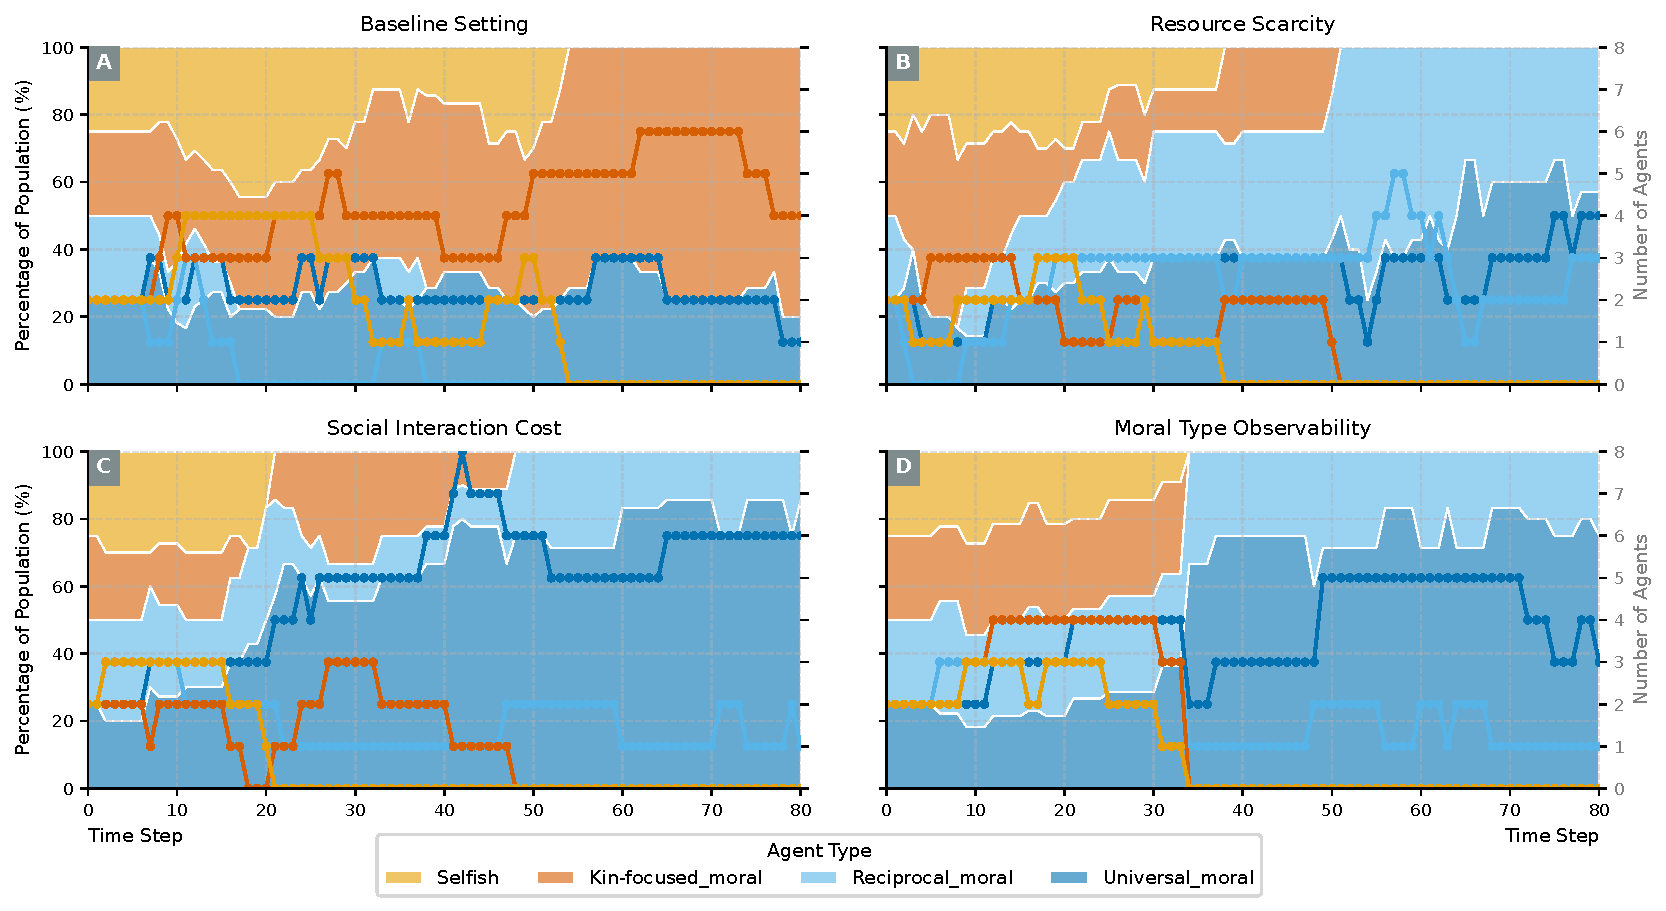
\includegraphics[width=\textwidth]{figures/population_grid_4panel.pdf}
    \caption{Population dynamics across four experimental settings, each showing a representative run where the most frequently dominant moral type in that setting prevails. Each panel displays the proportion (stacked area) and count (line) of surviving moral types over 80 simulation steps. (A)~Baseline: kin-focused agents dominate, leveraging efficient intergenerational HP transfer within families. (B)~Resource Scarcity: reciprocal agents dominate through coordinated coalition hunting. (C)~High Social Interaction Cost: universal agents emerge as dominant, as their cooperation does not require multi-round negotiation. (D)~Moral Type Unobservable: universal and kin agents coexist while reciprocal agents decline due to moral type misattribution. Note that outcomes vary across runs; aggregate win counts over 20 replicate runs are reported in Table~\ref{tab:replicate_outcomes_main}.}
    \label{fig:population}
\end{figure*}

\begin{table}[t!]
\centering
\small
\caption{Run-level win counts across settings. A moral type ``wins'' if it survives at step~80; coexistence credits every surviving type.}
\label{tab:replicate_outcomes_main}
\begin{tabular}{l c c c c c}
\toprule
\textbf{Setting} & \textbf{N} & \textbf{Uni.} & \textbf{Rec.} & \textbf{Kin} & \textbf{Sel.} \\
\midrule
Baseline         & 8 & 3 & 2 & \textbf{6} & 2 \\
Resource Scarc.  & 4 & 2 & \textbf{3} & 0 & 1 \\
Social Int.\ Cost & 4 & \textbf{2} & 1 & 0 & 1 \\
Moral Observ.    & 4 & \textbf{4} & 0 & 2 & 0 \\
\bottomrule
\end{tabular}
\end{table}

\paragraph{Moral Evolution}
We run several exemplary experiments to demonstrate how moral dispositions interplay with various settings. To characterise stochastic variability, we execute the Baseline setting $N{=}8$ times and each ablation setting $N{=}4$ times (20 runs total) using distinct random seeds. Table~\ref{tab:replicate_outcomes_main} summarises the run-level outcomes; population trajectories for all runs appear in the supplement (\S\ref{sec:replicates}).
Each simulation is initialized with 8 agents (2 per moral type). Representative population trajectories for four experimental settings are shown in Fig.~\ref{fig:population}; cross-model statistics for the baseline are reported in Table~\ref{tab:cross_model}.

\textbf{Baseline:} With abundant resources, low social cost, and observable moral types, kin-focused agents dominate (6/8 runs). They benefit from a compact cooperation unit---the family---that avoids the overhead of broader alliances while rapidly producing offspring.

\textbf{Resource Scarcity:} When resources are scarce, reciprocal agents dominate (3/4 runs) through coordinated coalition hunting. Kin-focused agents fail because reproduction costs 10 HP while offspring are born at only 2--3 HP, creating a recovery gap that parents cannot bridge under scarcity---the same allocation mechanism that powers kin dominance in the Baseline becomes a lineage-level death sentence when resources are tight.

\textbf{High Social Interaction Cost:} With only 1 social round before production, universal agents emerge as the most viable type (2/4 runs). Their cooperation does not depend on negotiating explicit reciprocal contracts: they default to unconditional contribution even when there is no room to ratify exchanges. Reciprocal agents cannot set up the trust-verification cycle their strategy requires. Selfish agents collapse early, and kin-focused lineages cannot sustain themselves without cross-kin alliances. One run ends in reciprocal/selfish coexistence and one in full extinction---indicating that unconditional cooperation is the most reliable, though not the only, viable strategy under low-bandwidth conditions.

\textbf{Moral Type Unobservable:} When agents cannot directly observe moral types, kin and universal agents survive while others decline (universal survives in all 4 runs). Reciprocal agents fail because their cooperative behaviours are misinterpreted as selfish, triggering exclusion from coalitions. This demonstrates that the ability to signal one’s moral type is critical for conditional cooperation strategies. Detailed per-setting results and mechanistic case studies are provided in the Appendix (\S\ref{sec:case_studies}).

\begin{figure}[t!]
    \centering
    \begin{subfigure}[b]{0.9\columnwidth}
        \centering
        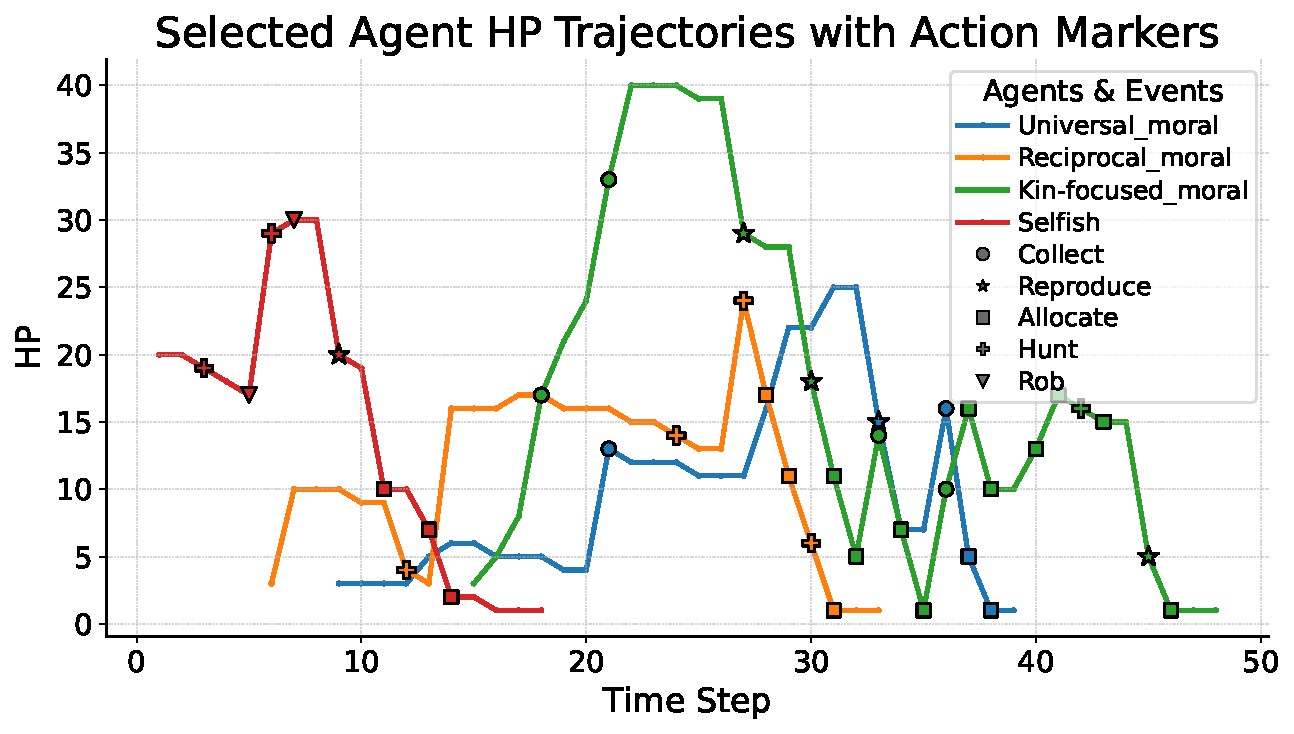
\includegraphics[width=\linewidth]{figures/agent_hp_with_action.pdf}
        \caption{HP trajectories of example agents.}
    \end{subfigure}
    \begin{subfigure}[b]{0.9\columnwidth}
        \centering
        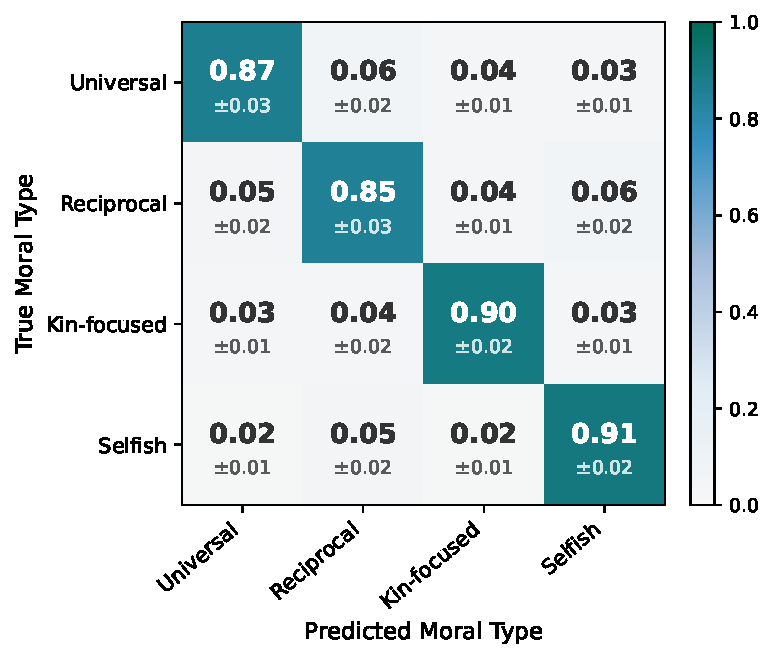
\includegraphics[width=\linewidth]{figures/multi_run_confusion_matrix.pdf}
        \caption{Confusion matrix of moral type inference (averaged over 8 runs).}
    \end{subfigure}
    \caption{Validation results of the baseline simulation.}
    \label{fig:validation}
\end{figure}

\begin{table}[t]
\centering
\small
\begin{tabular}{@{}lccc@{}}
\toprule
\textbf{Sim.\ Model} & \textbf{CM Diag.\ Acc.} & \textbf{Dom.\ Type} & \textbf{Final Pop.} \\
\midrule
GPT-5-mini & $0.89 \pm 0.03$ & Kin (6/8) & $12.0 \pm 2.0$ \\
Qwen-3.5 & $0.86 \pm 0.03$ & Kin (7/8) & $11.6 \pm 1.7$ \\
Kimi-K2.5 & $0.87 \pm 0.03$ & Kin (5/8) & $12.1 \pm 1.8$ \\
\bottomrule
\end{tabular}
\caption{Cross-model robustness of the baseline simulation over 8 independent runs per model. CM Diag.\ Acc.\ = confusion-matrix diagonal accuracy.}
\label{tab:cross_model}
\end{table}

% \begin{figure}[ht]
%     \centering
%     
\includegraphics[width=0.8\columnwidth]{figures/action_distribution_across_cases.pdf}
%     \caption{Action proportion across experiment settings}
%     \label{fig:ablations}
% \end{figure}

\paragraph{Simulation Validation}
We validate the simulation from both environmental feedback and morality-behavior consistency perspectives.
For environmental feedback, we plot HP trajectories alongside actions for representative agents in Fig.~\ref{fig:validation}~(a). The kin-focused agent illustrates strong familial bonds: born at step~15 with 3~HP, it gained HP through collection, produced two offspring, and frequently shared resources with family before eventually dying from insufficient energy recovery after a third reproduction.
To verify morality-behavior consistency, we employ a separate, more capable model (GPT-5) as an evaluator to infer each agent's moral type from observed behaviors. Fig.~\ref{fig:validation}~(b) shows the confusion matrix averaged over 8~runs, achieving a diagonal accuracy of $0.89 \pm 0.03$, confirming that agents behave consistently with their assigned moral dispositions. As shown in Table~\ref{tab:cross_model}, this strong alignment is consistent across all tested simulation models.

\paragraph{Robustness and Ablation Analysis}
To assess the contribution of each cognitive module in \agentframe and the sensitivity to prompt wording, we conduct controlled ablation and prompt-variation experiments (Table~\ref{tab:ablation}). Removing any single module degrades behavior-morality alignment, with long-term memory showing the largest impact ($-0.11$). Stripping all modules (ReAct baseline) reduces diagonal accuracy to $0.67$, confirming that each component contributes meaningfully beyond standard LLM reasoning. Prompt sensitivity tests using two semantically equivalent rewrites show negligible variation ($\leq 0.03$), indicating that our conclusions are robust to surface-level prompt wording rather than artifacts of specific phrasing.

\begin{table}[t]
\centering
\small
\caption{Architecture ablation and prompt sensitivity analysis. All experiments use the baseline configuration with GPT-5-mini.}
\begin{tabular}{@{}lcc@{}}
\toprule
\textbf{Condition} & \textbf{CM Diag.\ Acc.} & \textbf{$\Delta$} \\
\midrule
Full Architecture & $0.89 \pm 0.03$ & --- \\
\midrule
\multicolumn{3}{@{}l}{\textit{Architectural Ablation}} \\
\quad w/o Memory & $0.78 \pm 0.04$ & $-0.11$ \\
\quad w/o Plan & $0.82 \pm 0.04$ & $-0.07$ \\
\quad w/o Reflection & $0.84 \pm 0.03$ & $-0.05$ \\
\quad ReAct Baseline & $0.67 \pm 0.06$ & $-0.22$ \\
\midrule
\multicolumn{3}{@{}l}{\textit{Prompt Sensitivity}} \\
\quad Variant A (lexical rewrite) & $0.87 \pm 0.03$ & $-0.02$ \\
\quad Variant B (structural rewrite) & $0.86 \pm 0.04$ & $-0.03$ \\
\bottomrule
\end{tabular}
\label{tab:ablation}
\end{table}

\paragraph{Mini-game}
We constructed an example mini-game to study how morality interacts with other factors for a resource allocation scenario within family. More examples are in the Appendix.

To understand how moral dispositions shape resource sharing within families, we studied intergenerational transfers between parents and children. Our experiment involved parent-child dyads from two distinct life stages: young parents with infants and elderly parents with adult children. We modeled four moral dispositions—reproductive selfishness, universal group-focus, reciprocal group-focus, and kin-focus—creating eight unique scenarios. For each, we generated a heatmap to visualize parental transfer behavior. In these maps, the x- and y-axes represent the parents' and child's health (HP), respectively, while the color indicates the amount of resources transferred. The results reveal that provisioning strategies are systematically driven by moral type, showing clear thresholds for initiating aid, different sensitivities to self versus offspring health, and complex interactions between moral orientation and age.

As shown in Fig.~\ref{fig:allocate_kinaltru}, parents generally transfer surplus health points (HP) to their children. This behavior is strongly modulated by age, with older parents allocating significantly more resources as they approach their lifespan limits. Moral dispositions, however, introduce the most striking variations. For instance, reproductively selfish parents tend to hoard resources for self-preservation, while in stark contrast, kin-focused parents consistently prioritize their offspring. In extreme cases, these kin-focused parents sacrifice nearly all of their own HP to ensure their child's survival and fitness.

\begin{figure}
    \centering
    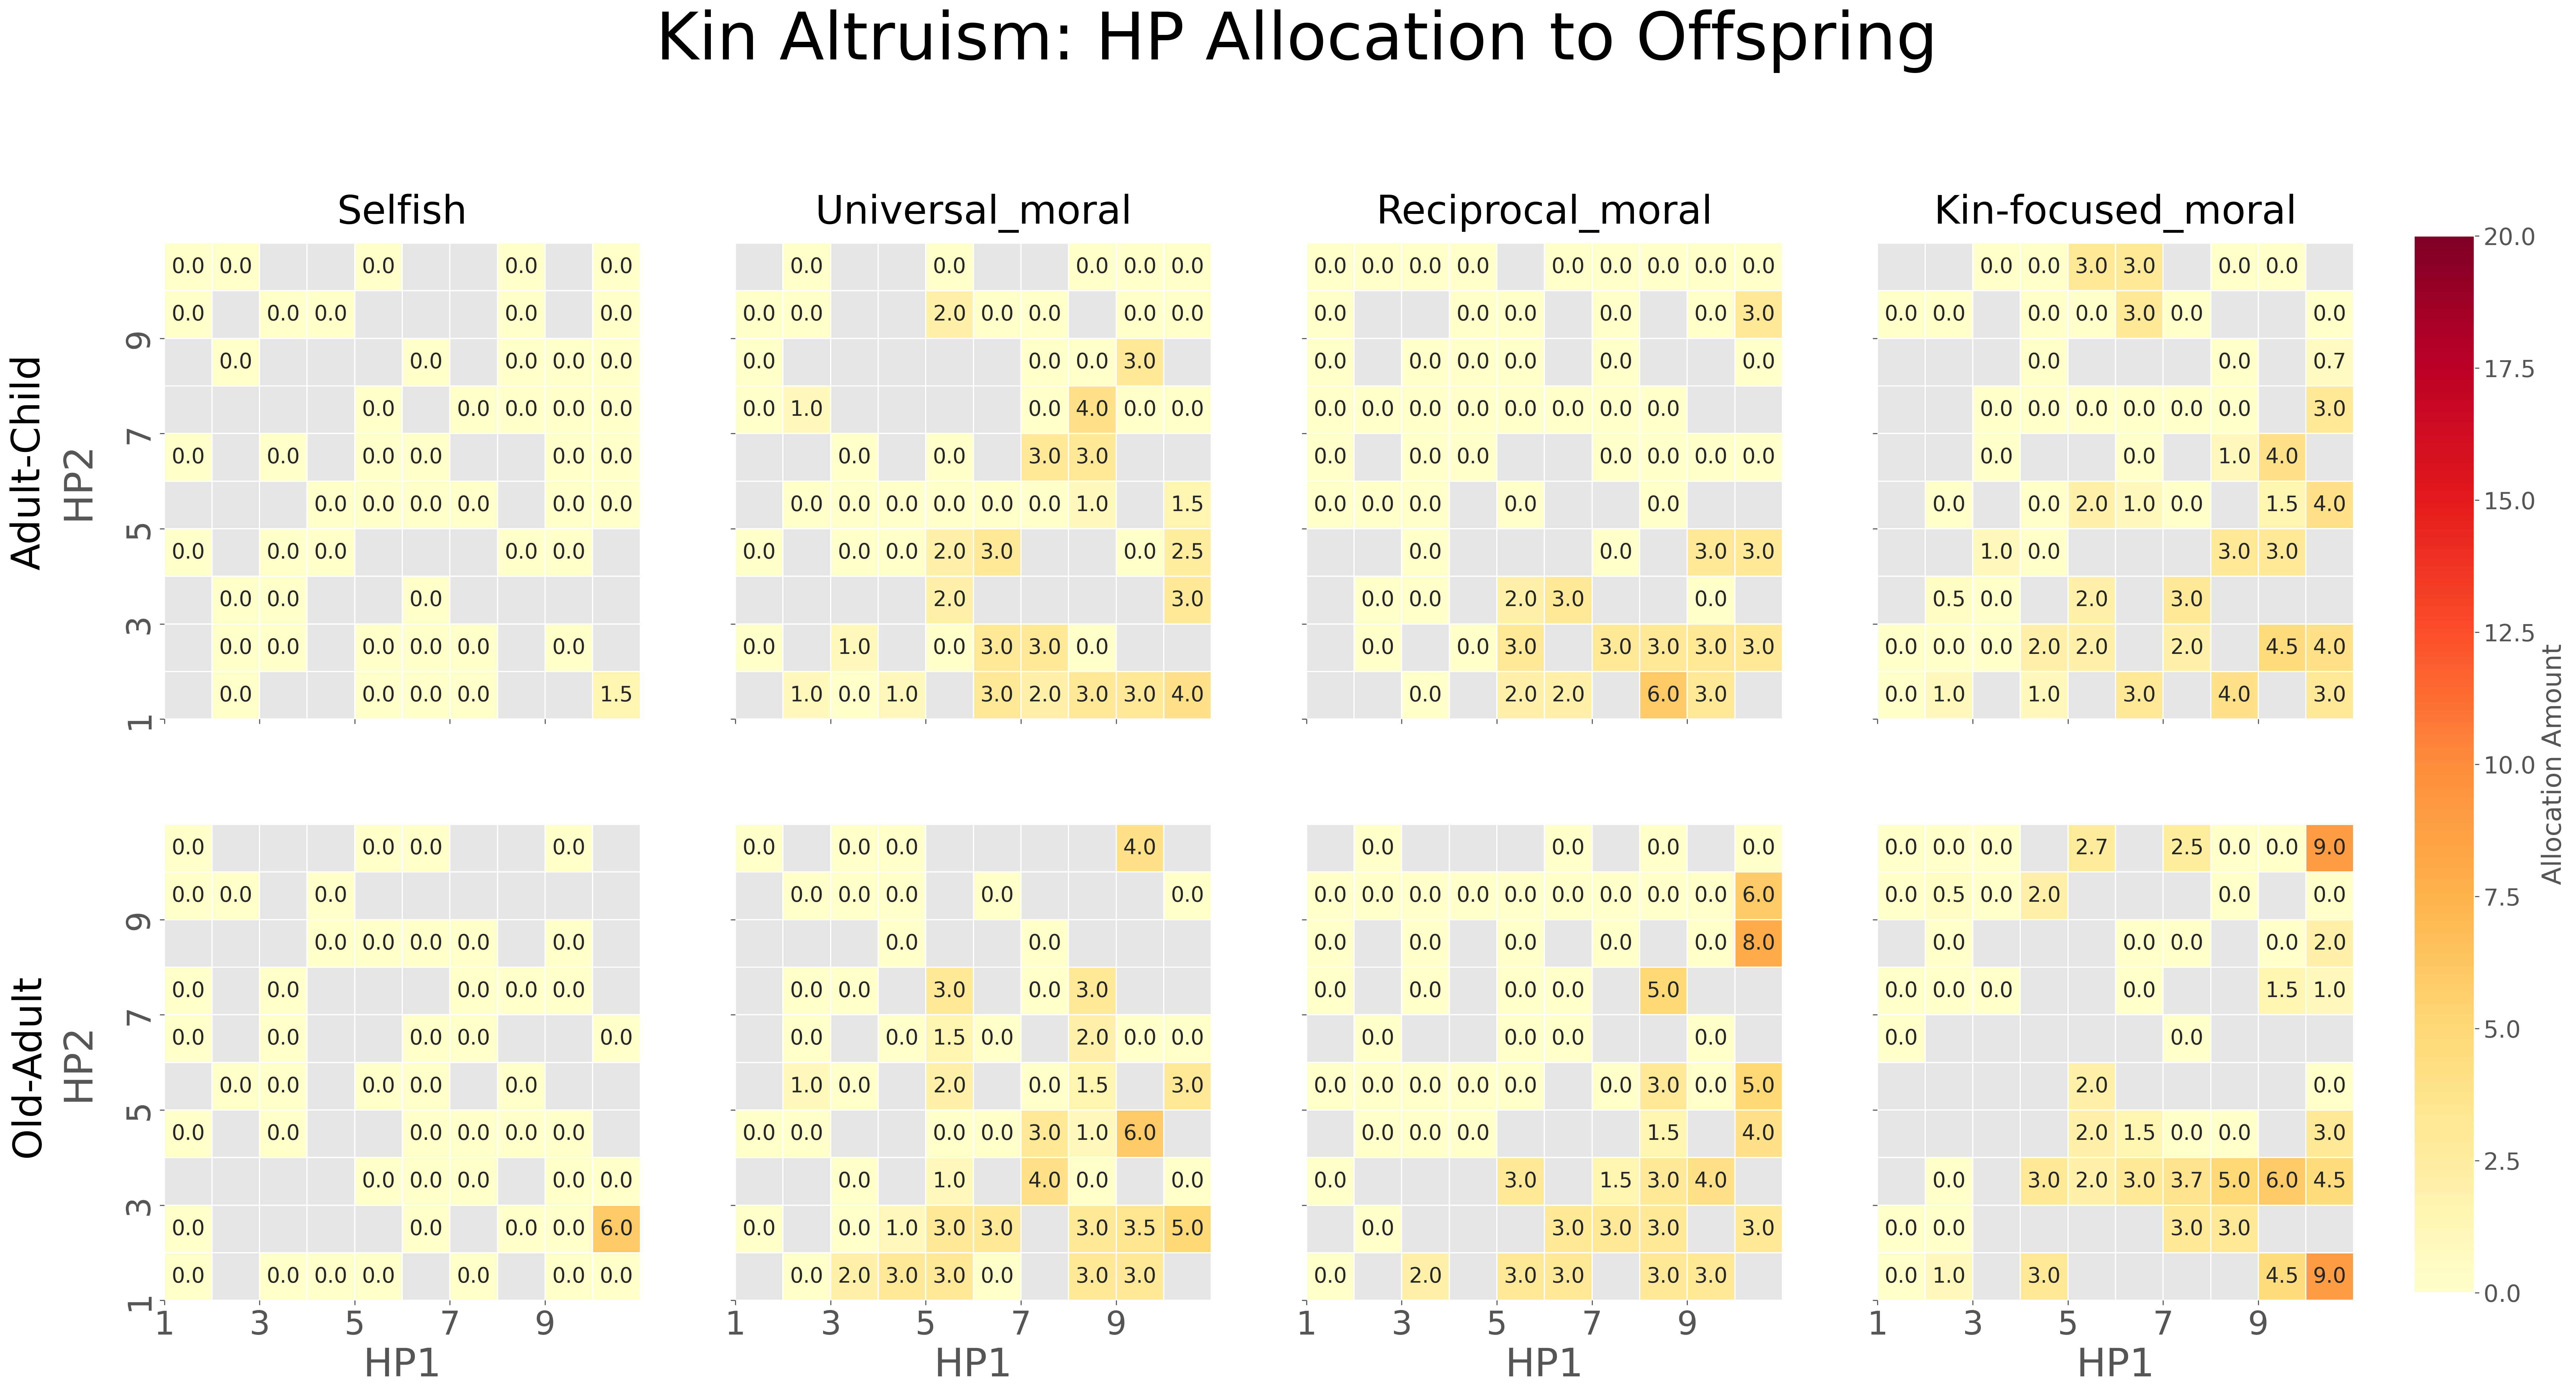
\includegraphics[width=\linewidth]{figures/allocation_heatmaps.png}
    \caption{Kin Altruism: A Minigame on Family Resource Allocation.}
    \label{fig:allocate_kinaltru}
\end{figure}

\paragraph{Importance of Cognitive Constraints}
Our simulations highlight the critical role of cognitive constraints in moral evolution---a factor rarely emphasised by prior theories. When communication bandwidth is severely limited, conditional cooperation strategies (reciprocal morality) collapse because they cannot complete the negotiation cycles their strategy requires; under these conditions, universal morality---which does not depend on explicit contracts---emerges as the most viable strategy, while selfish agents still decline due to social exclusion (Fig.~\ref{fig:population}, Table~\ref{tab:replicate_outcomes_main}). This pattern exemplifies bounded rationality~\citep{simon1991bounded} and supports the Morality-as-Cooperation theory~\citep{Curry2019MAC}, which posits that morality evolved to facilitate cooperation. We further observe that many conflicts stem from misunderstandings due to limited behavioural cues, consistent with information transmission limits~\citep{shannon1948mathematical, deutsch1973resolution}. Universal agents, while risking exploitation, gain an advantage by avoiding misinterpretation, connecting to theories of reputation and costly signalling~\citep{alt1988reputation, gintis2001costly, nowak2005evolution}.


\paragraph{Connections to Established Theories}

The results capture phenomena aligning with diverse established theories, validating our framework’s ability to produce meaningful and insightful results.


\textit{Altruism Promotes Group-level Survival:}
Consistent with foundational theories of social evolution~\citep{hamilton1964genetical,trivers1971evolution,boyd1987evolution,nowak1998dynamics}, our simulations demonstrate that moral agents generally enhance group-level survival across all settings (Fig.~\ref{fig:population}, Table~\ref{tab:replicate_outcomes_main}), while selfish agents are strongly disfavoured. The specific form of morality that prevails depends on environmental conditions---broader cooperation becomes more advantageous as pressures intensify.


\textit{Moral Evolution in Prehistoric Societies:} 
We observed that agents with a broader moral scope do not always prevail. Specifically, kin-focused agents tend to be more stable: it always becomes the type of agents lasting to the end except for a high social interaction cost scenario (Fig.~\ref{fig:population}). This finding resonates with anthropological evidence from matrilineal prehistoric societies~\citep{holden2003matriliny, mattison2011evolutionary, wang2023ancient} and with theories proposing that the unambiguous biological connection of maternal relationships formed a reliable foundation for early human cooperation~\citep{hamilton1964genetical}.

\textit{Other Theories:}
We observe that universal moral agents often get exploited by less moral agents in the simulation, illustrating altruistic punishment’s role in cooperation maintenance~\citep{fehr2002altruistic}. Sometimes the agents choose the wrong time to reproduce because they see other agents' reproduction activities, connecting with social learning theory~\citep{bandura1977social}. Appendix includes a comprehensive list of theoretical connections.

